\section{Exact score: the threshold is where the theory puts it}
\label{sec:exact}

\paragraph*{Setup.}
The data are eight Gaussian modes on a unit circle in the position plane, each with position standard deviation $s=0.08$, and with CLD initial velocities $v\sim\mathcal N(0,0.01)$; the phase space is four-dimensional.
We use the default CLD flow ($\kappa=2$), $\smin=0.005$ and $\smax=40$.
The total blur is the same for every $r$: $T=\ln(\smax/\smin)/r$.
The score of the forward mixture is computed exactly.
Samplers \Sa{} and \Sb{} are \emph{paired}: they share the prior draw and the Brownian increments.
Each run uses $N=40\,000$ samples, five seeds and two step sizes ($h\approx0.002$ and $0.001$), combined by Richardson extrapolation (App.~\ref{app:methods}).
The measured quantity is the log ratio $L$ of the within-mode position variance to its target, the data blurred by $\smin$; it is computed per mode, with modes assigned to the nearest centre, and pooled.

\begin{observation}
\label{obs:threshold}
For $r<\kappa$ the clipped sampler shrinks the within-mode variance relative to \Sb{}: by $100L=-1.17$ at $r/\kappa=0.5$, falling to $-0.10$ at $0.95$ [Fig.~\ref{fig:threshold}].
For $r\geq\kappa$ the difference is exactly zero (Proposition~\ref{prop:exact}).
Fitting the one-mode theory curve with a free amplitude and a free threshold to the points with $r<\kappa$ gives $\kappa_{\rm fit}/\kappa = 0.992 \pm 0.025$ (bootstrap over seeds, 16--84\%: $[0.968, 1.005]$).
A model-free quadratic fit gives $0.995$ $[0.978, 1.030]$.
Samplers \Sb{} and \Sc{} return the target variance at every $r$ ($|100L|\leq 0.5$).
\end{observation}

Fitting is needed because the shrinkage vanishes linearly at $\kappa$ and is hidden by noise just below it: at $r/\kappa=0.95$ it is not distinguishable from zero with five seeds.

\begin{observation}
\label{obs:amplitude}
The amplitude is $0.76\pm0.07$ of the one-mode Gaussian theory (Proposition~\ref{prop:exact} applied to a single mode).
For a single isolated mode the same pipeline agrees with the theory to within 1\%.
When the circle radius is doubled, quadrupled and multiplied by eight, the ratio rises to $0.80, 0.95, 0.98, 0.98$ (radius $\times1$, $\times2$, $\times4$, $\times8$; three seeds each).
The shortfall is therefore caused by the neighbouring modes.
About 7.7\% of the trajectories end in a different mode under \Sa{} than under \Sb{}; this widens the spread between seeds but does not account for the mean shortfall.
\end{observation}

\begin{figure}[t]
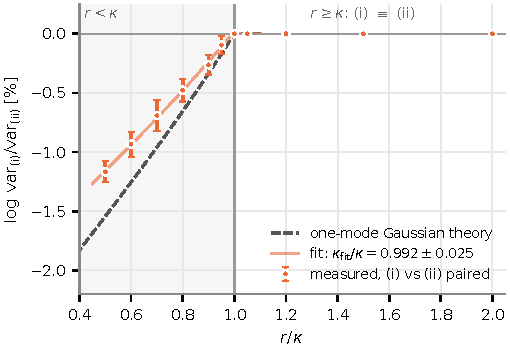
\includegraphics[width=\columnwidth]{figures/fig1_threshold}
\caption{Within-mode variance of the clipped sampler \Sa{} relative to the corrected sampler \Sb{} (paired), with the exact score, for the default CLD flow ($\kappa=2$) and eight Gaussian modes.
Points: mean $\pm$ s.e.\ over five seeds, step-extrapolated.
Dashed: one-mode Gaussian theory.
Solid: the theory with a fitted amplitude and threshold.
For $r\geq\kappa$ the two samplers are the same equation.}
\label{fig:threshold}
\end{figure}
